\chapter{Experiments and Results}
\label{chap:experiments}

Experiments for our VMMR system are conducted on a platform with Dual-Core Intel Core i5 (2.9 GHz), 16 GB 1867 MHz DDR3 and MATLAB R2019b.

\section{Pre-processing}
\label{sec:pre-processing}
In the pre-processing stage, Regions Of Interest (ROI) are cropped out, converted to grayscale and scaled to a unified resolution of 140-by-140.

\subsection{Duplicates Removal}
The original dataset contains $2117$ frontal car images in total. 
However, for each distinct car in the dataset, there exist multiple variations, which typically include a coloured non-cropping version, a grayscale downsampled version, as well as a grayscale downsampled and ROI-cropped version.
Duplicates removal are achieved by preversing the coloured non-cropping version of size 640-by-480 only among those variations.
A total of $500$ "original images" are retrieved.

For "peugeot306" and "citroen\_saxo" classes, however, the coloured non-cropping versions are missing.
In that case, the grayscale downsampled and ROI-cropped versions are chosen and both the cropping and converting steps are skipped.


\subsection{Cropping}
In the cropping stage, ROI are cropped out from the "original images".
Locations of number plates in the "original images" have already been pre-labeled.
In this paper, ROI is defined in terms of the width $w$ and the center $(x_c, y_c)$ of the number plate in the image.
Concretely, the rectangle bounding box of ROI is written as $[(x_c-1.4w, y_c-0.7w), ((x_c+1.4w, y_c+0.4w))]$.
An example of ROI cropping is shown in Figure \ref{fig:roi}.

\begin{figure}
\centering
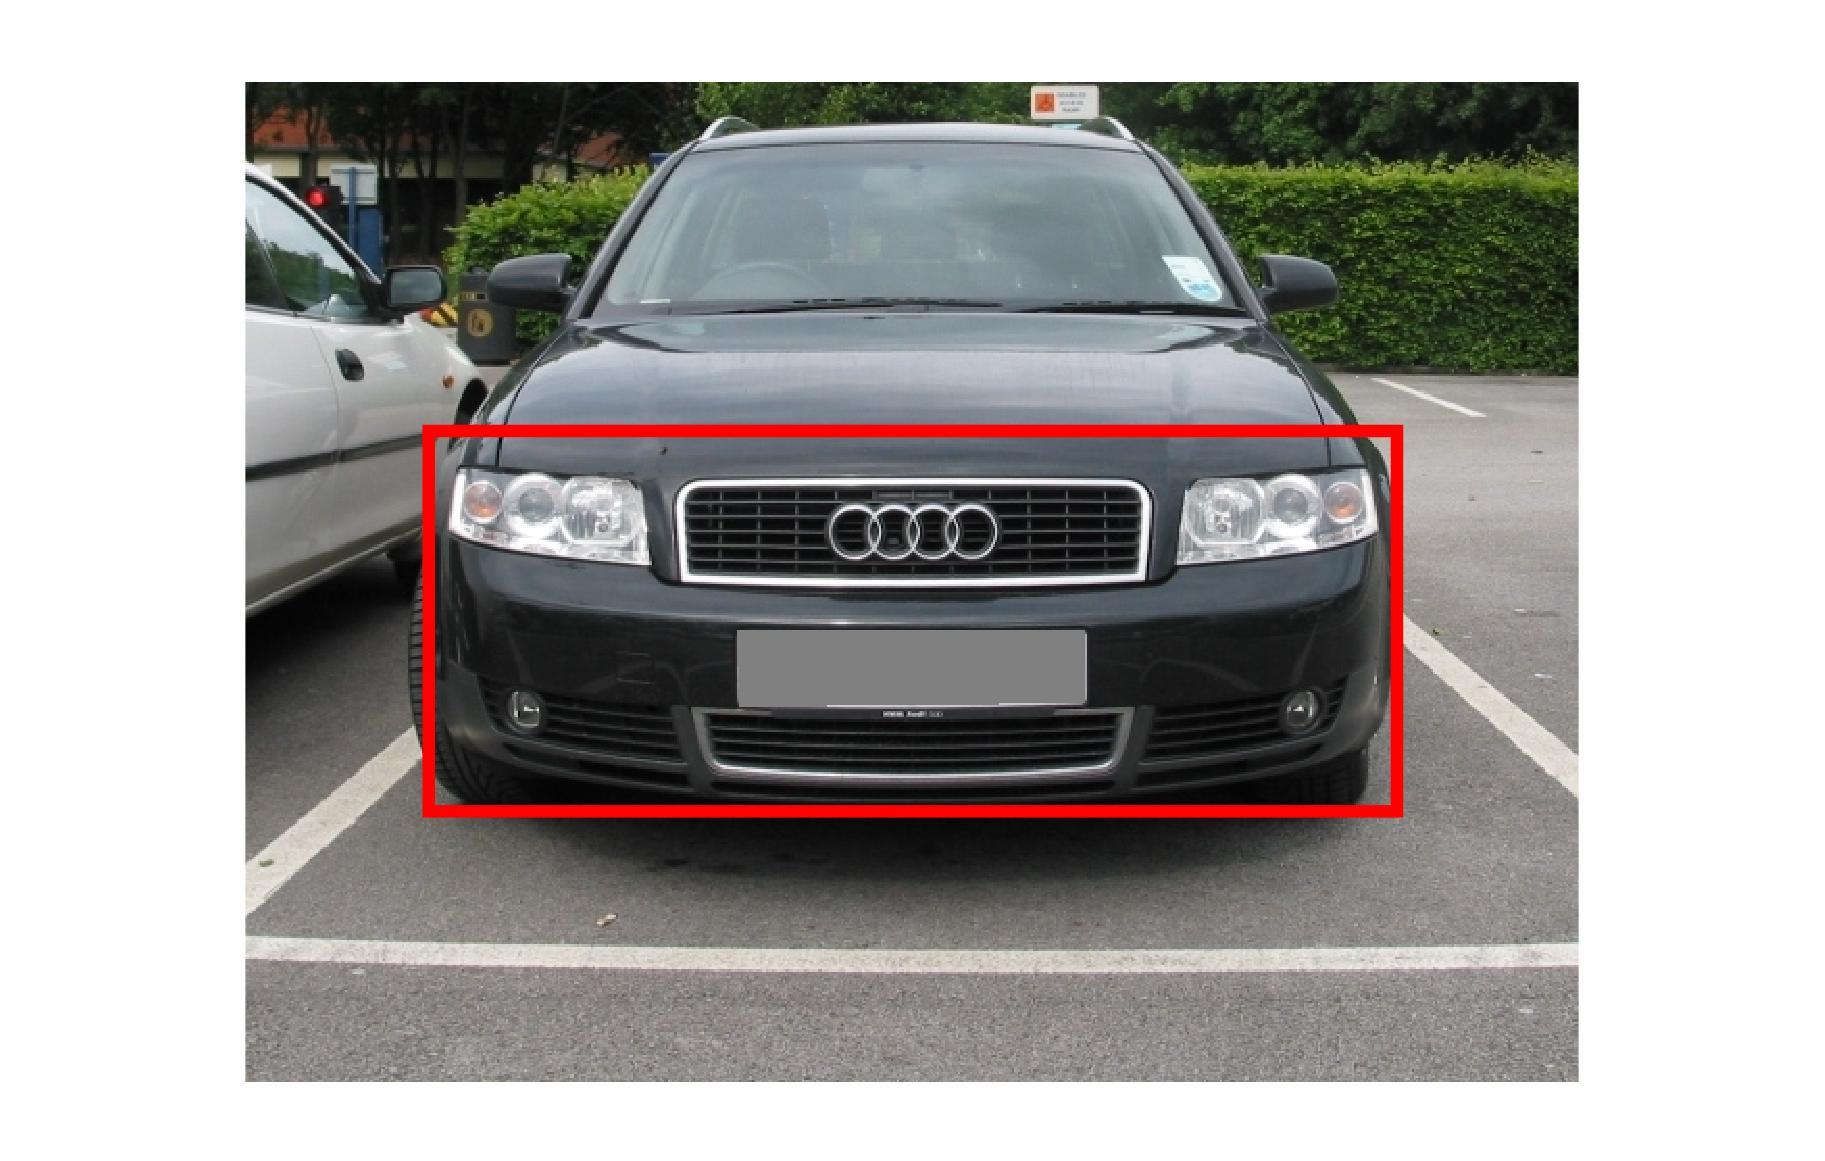
\includegraphics{roi}
\caption{An Example of ROI Cropping on a "Original Image" from "audi\_a4" Class.}
\label{fig:roi}
\end{figure}


\subsection{Converting to Grayscale}
The cropped RGB images are convertted to grayscale image using Formula \ref{eq:rgb2gray}.

\begin{equation}
\label{eq:rgb2gray}
I = 0.2989 R + 0.5870 G + 0.1140 B
\end{equation}

The pre-processed dataset before scaling can be retrieved from GitHub \footnote{https://github.com/daidahao/COP507-Vehicle-Make-Model-Recognition/tree/master/dataset}.

\subsection{Scaling}
All images are scaled to a unified resolution of 140-by-140 at runtime.
A set of scaled image samples for all classes are presented in Figure \ref{fig:classes}.

\section{Cross-Validation}

% \section{Merits of Performance}

\section{Effects of Features Extraction Methods}
\label{sec:effects-fe}

\section{Effects of Classification Methods}
\label{sec:effects-cls}

\section{Effects of Dimensionality Reduction Methods}
\label{sec:effects-dim}

